\documentclass{article}

\usepackage[final]{neurips_2021}
\usepackage{mwe}
\usepackage{graphicx}
\graphicspath{{./image/}}

\usepackage[colorlinks=true]{hyperref}
\usepackage{url}
\usepackage{enumitem}
    
\usepackage[utf8]{inputenc} % allow utf-8 input
\usepackage[T1]{fontenc}    % use 8-bit T1 fonts
\usepackage{hyperref}       % hyperlinks
\usepackage{url}            % simple URL typesetting
\usepackage{booktabs}       % professional-quality tables
\usepackage{amsfonts}       % blackboard math symbols
\usepackage{nicefrac}       % compact symbols for 1/2, etc.
\usepackage{microtype}      % microtypography
\usepackage{xcolor}         % colors

%Import the natbib package and sets a bibliography style
\usepackage{natbib}
%To change format of how references are cited, must use:
\setcitestyle{square,numbers}
\bibliographystyle{abbrvnat}


\title{HR Attrition Analysis}

\author{
  Anja Wu \\
%   Vector Institute\\
%   Mothers in Machine Learning\\
  %\texttt{anjaradakovic33@gmail.com} \\
  \vspace{-15mm} 
}

\begin{document}

\maketitle

\begin{abstract}
\vspace{-2mm} 
  Using an employee dataset from Kaggle, factors affecting attrition were studied, along with creating a model to predict attrition based on the employee features contained within the dataset. Several models and methods were tried to get maximum accuracy and deal with the imbalance of attrition feature. The best model was the decision tree, primarily when the oversampling method was used to randomly distribute the training data. A logistic regression was used to further understand any relationships between features and attrition. The top features which had the largest effects on attrition were: total working years, years at company, years with current manager, and percent salary hike.
  \vspace{-3mm} 
\end{abstract}





\section{Introduction}
\vspace{-2mm} 
% Discuss the type of problem you are trying to solve. Briefly discuss previous work in this area (if applicable). What is your hypothesis?
I am fairly new to analysis and have not worked with any HR analysis prior to this project but I will be looking at attrition in a company with specific employee features. Through the analysis of employee data using a Kaggle dataset \cite{kaggledata}, I will be trying to predict attrition of employees within a year at a company based on the data given. This dataset drew my interest given articles I have read online about the Great Resignation phenomenon that has arisen during the pandemic. The main goal is to understand what factors influence attrition the most and if there are any suggestions for the company to try to keep more of their employees. A secondary goal will be to find the best predictive model.

Two part hypothesis:
\begin{enumerate}[leftmargin=0.5cm]
\item There are several factors which will impact attrition the most: "EnvironmentSatisfaction", "JobSatisfaction", "PercentSalaryHike", and "YearsWithCurrManager". I think the best model to give me the relationship between the features and attrition is logistic regression. 
\item I think the decision tree model will lead to the best predictive model because of research that indicated it performs particularly well with imbalance outcomes. 
\end{enumerate}







\section{Problem Definition}
\vspace{-2mm} 
\label{headings}
% Describe the specific problem you are trying to solve and discuss why it is a challenge. Explore and describe the dataset you are using. Discuss your approach, model options, the model you chose, and why you selected it.
\paragraph{Problem:} Attrition in general is a difficult topic to predict because so many factors need to be considered. Even if you have the perfect model with all factors considered, people’s intent to leave changes on a variety of things that is based on personal preferences. This can make it difficult to extract a general rule for all people. Due to the vast variety of data in social science (such as this type of data), you would not expect the same level of correlation that you would want to see in other situations. It is enough to have a moderate correlation between any of your features and attrition to draw conclusions. It is all relative to the other features you have and how they perform. Analyzing attrition by looking at the correlations can help businesses adjust their company structure to retain as many personnel as possible because it gives more insight into the why. 

\paragraph{Dataset:} The dataset has personal information about the employee (age, gender, marital status, distance from office, etc.), work background of employee (education, number of companies worked, etc.), employee job information (job level, role, job performance, etc.), and job pay (monthly income, stock options, etc.).  The dataset also had whether the employee has left in the past year or not (attrition). When looking at attrition, not all attrition is the same; it is important to look at regrettable vs non-regrettable attrition. Because sometimes attrition can be good, if it is for people who aren’t in the right role to make the impact on what they are working on. This is something that should be looked at. This particular dataset only had job performance of 3 or 4, which is fairly high. So I went ahead with the assumption that they were only looking at their higher performers and what was causing them to leave. 

\paragraph{Data Pre-Processing:} During the pre-processing of data, there were several things found:
\vspace{-2mm} 
\begin{itemize}[leftmargin=0.5cm]
\item Several columns had only one possible option, this means they do not add any signal towards the analysis of attrition. I deleted these columns, so as to reduce dimensions.
\item The columns that had features that were categorical were encoded using a simple integer encoding, ranging from 0 to n-1 categories. There are many encodings to pick from and the simple integer encoding I chose was not the best one, but I chose it for simplicity sake to allow focus on the other parts of my project. 
\item When doing regressions, collinearity must be checked. The correlation matrix can be seen to have several variables that have a high correlation. The best way to deal with this is to check for multicollinearity using VIF. \cite{VIF1} \cite{VIF2}
\begin{itemize}
\item VIF runs a linear correlation for each feature against all other features
\item For the VIF calculations it can be seen that all values are below 5 implying that  features are not highly correlated. This means that we can proceed with our regression without dropping any columns.
\end{itemize}
\end{itemize}

Dealing with imbalance: Upon further exploration of the data, it was discovered that the attrition feature is imbalance (which makes sense). There are different methods to deal with imbalance and I found a good article  \cite{imbalance} that summarizes 10 ways. I chose the following methods:
\begin{enumerate}[leftmargin=0.5cm]
\item[a)] \underline{Random over-sampling with imblearn:} The imblearn library takes a random sample from the minority class, with replacement, until the number of samples is the same as the majority class.

\item[b)] \underline{Random under-sampling with imblearn:} The imblearn library takes a randomly generated sample of the majority class, in my case, without replacement, to match the number of samples in the minority class.

\item[c)] \underline{Synthetic Minority Oversampling Technique (SMOTE):} In general, SMOTE is an oversampling technique which uses k-nearest neighbours to increase the sample of minority class. It does this by taking k-nearest neighbours from a randomly selected minority point and then randomly selecting one of the neighbours. Then it creates a new synthetic point in between the minority point and its nearest neighbour. 
For this, I chose k =5. I tried a bunch of different k-values multiple times (5, 10, 15, 25, 30, 50, 100) and they all gave relatively the same predictive power. So for computational power and not risking overfitting, I chose the lowest k-value.

\item[d)] \underline{Under-sampling: Tomek links:} In general, Tomek links uses k-Nearest Neighbours to select for undersampling. The concept is that the algorithm will pair minority and majority points on the boundary that are a small distance from each other and will convert the majority label to the minority label. 
As can be seen in our data, the number of points that it converted was very minor, leading to still a great divide between the majority and the minority label. So this method was not a great one to be used for this dataset.

\end{enumerate}

\paragraph{Picking a model:} Through the course we learnt k-nearest neighbours, decision trees, random forests, linear regression, logistic regression, and forward-feed neural networks. In my initial goal of this project, seeing which features have the greatest effect on attrition, a regression would be the best bet. Regressions allow the analysis of the relationship between variables. A logistic regression is used when your outcome is binary and you would like to know to what degree your features affect the outcome.  I wanted to approach this problem to maximize the understanding of what factors lead to attrition, so I chose the logistic regression algorithm. Regression models allow the understanding of which features contribute the most to the outcomes you are looking for, this is done by looking at the coefficients. The accuracy of predictions was going to indicate to me how well the model predicted the importance of the features. A secondary goal of this project was to get as good of a predictive model to be able to predict whether an individual would leave the company based on the features inputted. 

Through research, I found that decision trees, in particular, usually perform the best with imbalance data. However, I still wanted to look at the relationship between the features and attrition, so I went ahead and did a logistic regression first. Then I also wanted to look at the best approach to see the difference in the performance, so I also did a decision tree. Random forest ensemble method would be a good idea to also use, however, I had found several drawbacks during my research\cite{RF-procon} \cite{why-RF} including being more of a black box, and having very little interpretability. So I discounted this method, due to the fact that a decision tree was said to perform quite well for imbalanced data and is slightly more interpretable than random forest. From there, I became curious and wanted to see how the k-nearest neighbours would perform compared to the other two models, since it did not stand out in the research for best inference nor best prediction of imbalance outcomes.

% So the three parts of the project are:
% AnjaWu\_P1\_LogRegres\_AttritionKaggle.ipynb
% AnjaWu\_P2\_DecisionTree\_AttritionKaggle.ipynb
% AnjaWu\_P3\_kNN\_AttritionKaggle.ipynb








\section{Model}
\vspace{-2mm} 
\label{others}
% Describe the details of your model and algorithm. Include your model as either a .ipynb file or as a shared Colab link embedded in your report.
Below I will be discussing how I designed the three models, keeping in mind that for all I used 5 different sampling methods to deal with the imbalanced data: no adaptation (this creates the baseline), random over-sampling with imblearn, random under-sampling with imblearn, Synthetic Minority Oversampling Technique (SMOTE), and under-sampling using Tomek links.

\subsection{Model 1: Logistic Regression}
\vspace{-2mm} %(AnjaWu_P1_LogRegres_AttritionKaggle.ipynb) 
Due to the correlation that I had found during the data exploration phase, I chose to try different variations of dropping correlated columns to analyze effects on the attrition outcome. Overall, I found not much of a difference when columns were dropped. In fact, the full dataframe performed better than having any potentially correlated features removed. So for all other methods of dealing with imbalance, I used the full dataframe. 

The data was separated into just training and testing sets, and the distribution of the labels was checked. After I fit the model using LogisticRegression() on the training set, I plotted the correlation coefficients for all features to get more of a visual of what features seemed to have the greatest effect. A confusion matrix was created to display the precision, recall, F1-score, and accuracy of the predictions. After this was done on all 5 methods (listed above), I created a table which held all results (highest correlation coefficient features and the metrics associated with the methods) to be able to more easily compare the different approaches. 

\subsection{Model 2: Decision Tree}
\vspace{-2mm} %(AnjaWu_P2_DecisionTree_AttritionKaggle.ipynb)
I modified the split data function we had in assignment two to work for this dataset. The function splits the data into 3 sets: training, validation, and test. The hyperparameters will be tuned using the training and the validation set, to only be tested once on the test set once the hyperparameters have been chosen. A select model function has been created (similar to assignment 2) which fits the tree onto the training data for various depths, and criterion and returns the accuracy (using the get\_acc function) for both the training and validation set.

Like before, the distribution of the attrition labels was analyzed for each method. Then the select model function was used to run different depths, using both Entropy and Gini criterion. The validation set accuracy was plotted along with the training set accuracy for those sets of depths and criterion. This was run 10 times to find an approximate best depth and criterion for each sampling method to be considered the best model (in the code, after each method, there is a description of why each was chosen). I fit the model using DecisionTreeClassifier() on the training set. Like before, a confusion matrix was created to check the accuracy, precision, recall, and F1-score for the final model chosen. Each method had a decision tree created, \textit{pictures are attached in the upload of the assignment.} 

\subsection{Model 3: k-Nearest Neighbours} 
\vspace{-2mm} 
This model uses a similar function to split the data into training, validation, and test sets as model 2. Also like before, the distribution of the attrition labels was analyzed for each method. A heatmap is displayed to show how closely related the training set is to the validation set. For this heatmap, it is better the closer the sets are to one another to better classify the data. I used a for loop to collect and plot all validation and training set accuracy to determine which number of nearest neighbours (k) should be used. Once the ideal k was selected for each method, I fit the model using KNeighborsClassifier(n\_neighbors=k) on the training set. Also like before, a confusion matrix was created to check the accuracy, precision, recall, and F1-score for the final model chosen. 

\section{Results and Findings}
\vspace{-2mm} 
% Present your results and interpret the outcome of your modeling. You should address whether your model answers the questions you described in your introduction. Talk about the practical applications and implications of your findings.


\subsection{Model 1: Logistic regression}
\vspace{-2mm} 
As can be seen in table \ref{table:1}, the method that lent the best predictions was the undersampling method because it has the best metrics (fair accuracy and has the best precision and recall), which I believe makes the ordering of the features the most likely to tell the story about which ones are the most important. In analyzing the regression coefficients, the most influential factors were: 
\begin{itemize}[leftmargin=0.5cm]
\vspace{-2mm} 
\item The more years worked, the less likely the individual was to leave
\item The more years spent at company, the less likely the individual was to leave
\item The more years with current manager, the less likely the individual was to leave
\item The higher the individual's salary increase, the more likely they are to leave the company
\end{itemize}
It is also interesting to note that individuals who work in sales have a much higher tendency to leave. 
\textit{*There is more of a breakdown for each method and coefficient in the .ipynb file.}

\vspace{1mm} 
\begin{table}[ht]
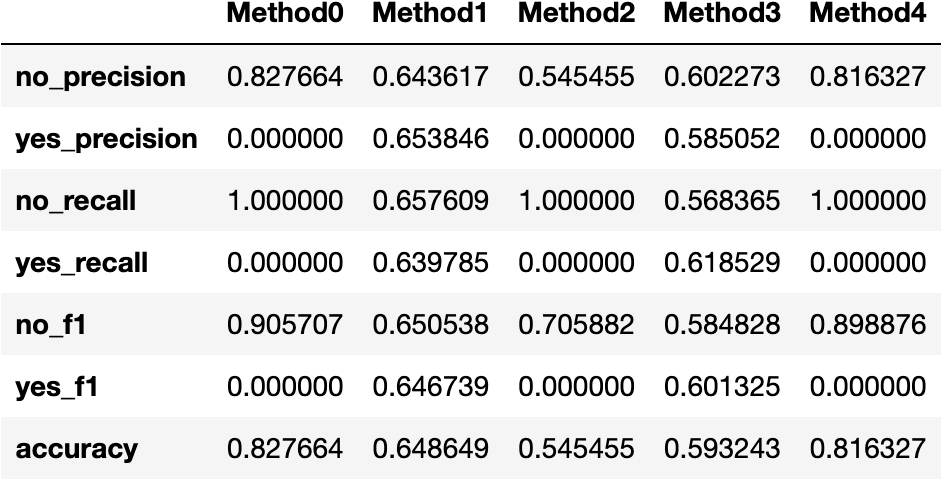
\includegraphics[width=13cm, height=6cm]{regression_coefficient_comparison.png}

\caption{Summary of the top 9 logistic regression coefficients for each method, along with the precision, recall, F1-score, and accuracy.}
\label{table:1} 
\vspace{-4mm}%Put here to reduce too much white space after your table 
\end{table}

This model did a good job in showing the relationship between our features and the attrition outcome. The next model, we will be trying to increase prediction - instead of focusing on the inference.



\subsection{Model 2: Decision Tree}
\vspace{-2mm} 
As can be seen in table \ref{table:2}, all methods for a decision tree are significantly better at predicting than the logistic regression. In particular, method 1 (random oversampling) performed the best, followed closely by method 3 (SMOTE). It seems that in general the oversampling is what made the predictions better. In analyzing the decision trees created, it was very clear that the data is not sorted according to the most correlated feature to attrition, but rather the algorithm focuses on the most information gain at each split. The algorithm cares most about the final output/classification and not how it gets there, and there could be cases where the optimal tree isn't the one that learns the most at the beginning of the tree (splits at hierarchy don’t necessarily signify importance). So this model would not be best at determining relationships between our features and the attrition outcome.

\begin{table}[htbp]
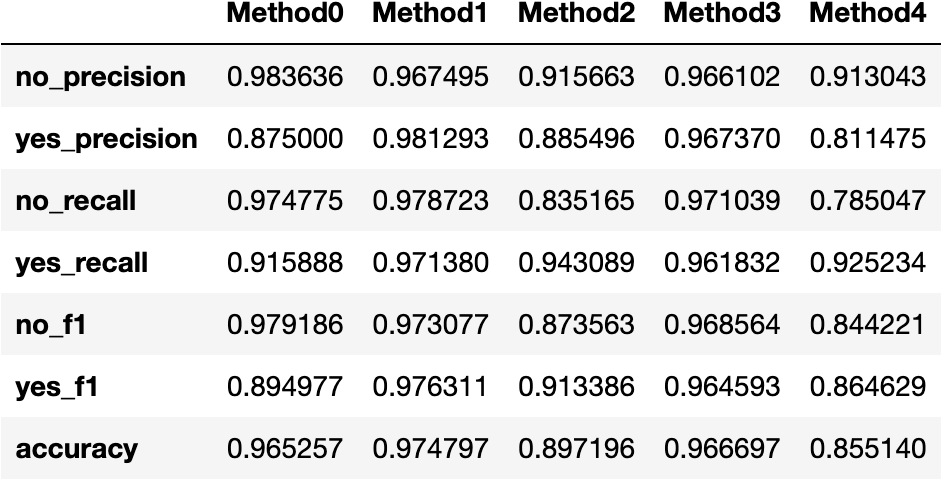
\includegraphics[width=8cm, height=3cm]{decision_tree_comparison.png}
% \vspace{1mm} 
\caption{Summary of the metrics (precision, recall, F1-score, and accuracy) for the different methods for the decision tree model.}
\label{table:2} 
\vspace{-4mm}%Put here to reduce too much white space after your table 
\end{table}






\subsection{Model 3: k-Nearest Neighbours}
\vspace{-2mm} 
As can be seen in table \ref{table:3}, most of the methods for a k-NN are worse at predicting than the decision tree and only slightly better than logistic regression, with the exception of method 1 (random oversampling). The random oversampling method with k-NN did a relatively good job at predicting both yes and no attrition, meaning it was successful in achieving the goal of predicting our attribute labels.
\begin{table}[h]
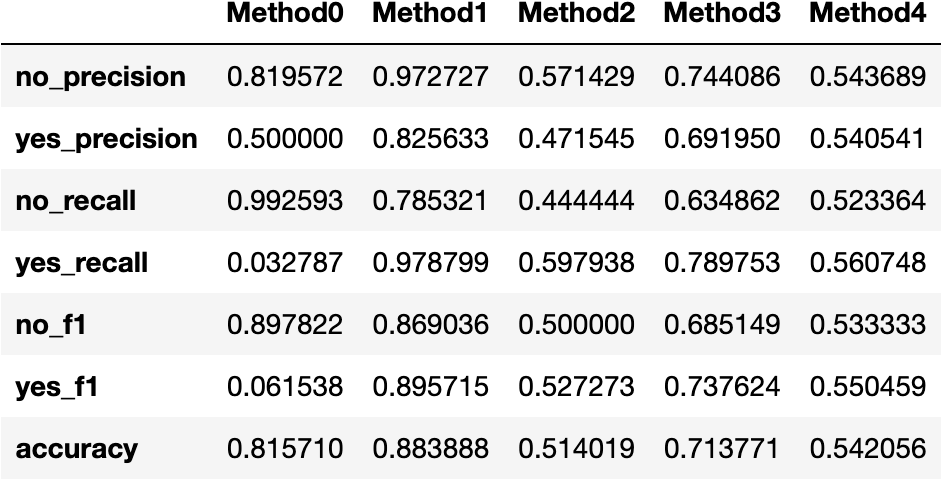
\includegraphics[width=7cm, height=3cm]{knn_comparison.png}
\vspace{2mm} 
\caption{Summary of the metrics (precision, recall, F1-score, and accuracy) for the different methods for the k-Nearest Neighbours.}
\label{table:3} 
\vspace{-7mm}%Put here to reduce too much white space after your table 
\end{table}

\paragraph{Real life application:} Finding the relationship between features and attrition can be useful to the company if we are looking at features that they can influence. For things such as total working years and years at the company, not much can be done. However, it would be good for the company to further explore the “why” behind more employees with high salary hikes leaving and if there is anything that can be done to get those individuals to stay (since they are most likely the higher performing employees). 

In terms of the predictive capabilities of the decision tree, it might be worthwhile to analyze out of certain employees that are instrumental to your organization, what is the likelihood of them leaving. Having a model that can predict an individual leaving, would be very useful in knowing where to focus efforts in getting high impact employees who might be close to leaving to stay.










\section{Conclusions and Future Work}
\vspace{-2mm} 
% Make inference from your project and discuss the limitations and strengths of your work, including fairness considerations. Discuss future opportunities.
Overall, logistic regression should be used to find relationships between features and the class (attrition). In this case, although the accuracy of prediction was not high, we can see some relationships between years worked, years spent at the specific company,  percent salary hike, and years with the current manager all impact attrition. For the best predictive model, I would recommend using the decision tree with the random oversampling method to deal with imbalance, as it gave the greatest overall accuracy (precision, recall, and F1-score). 

\paragraph{Limitations/Future Opportunities:}

\begin{itemize}[leftmargin=0.5cm]
\vspace{-1mm} 
    \item The encodings for the categorical data were done using simple encoding. I would consider exploring different encodings based on the type of data we are encoding. Pulling a pattern from “marital status” would be a different encoding than something like “job role”. These should not have been encoded using 0 to n-1 due to the fact that they are not ordinal. One fix would be to potentially use one hot encoding. 
    \item The p-values should have been analyzed more closely for the coefficients of the logistic regression to gauge the statistical significance of the features.
    \item One final limitation is that I do not have much HR experience and I might be missing some key fairness considerations in this domain/context.
\end{itemize}

\paragraph{Strengths:} 
\begin{itemize}[leftmargin=0.5cm]
\vspace{-1mm} 
    \item The distributions of the features were checked, which is important for checking for fairness. In general, there seemed to be no major imbalance in the features
    \item More than one model and method was used to see which would perform best with the dataset
    \item More than one run of each method and model was run to find an average (similar to bagging) for hyperparameters
\end{itemize}





\bibliography{refs} 


\newpage
\appendix

% \section{Appendix}

% Below are the accuracy plots for the decision tree and k-NN that can be found in the .ipynb.

% \subsection{Accuracy plots:}
% \subsubsection{Model 2: Decision tree}
% Method 0: Control

% \includegraphics[width=13cm, height=6cm]{DT_acc_plot_m0.png}

% Method 1: Random Over-Sampling

% \includegraphics[width=13cm, height=6cm]{DT_acc_plot_m1.png}

% Method 2: Random Under-Sampling 

% \includegraphics[width=13cm, height=6cm]{DT_acc_plot_m2.png}

% Method 3: SMOTE

% \includegraphics[width=13cm, height=6cm]{DT_acc_plot_m3.png}

% Method 4: Tomek Links

% \includegraphics[width=13cm, height=6cm]{DT_acc_plot_m4.png}

% \subsubsection{Model 3: kNN}
% Method 0: Control

% \includegraphics[width=13cm, height=6cm]{knn_acc_plot_m0.png}

% Method 1: Random Over-Sampling

% \includegraphics[width=13cm, height=6cm]{knn_acc_plot_m1.png}

% Method 2: Random Under-Sampling 

% \includegraphics[width=13cm, height=6cm]{knn_acc_plot_m2.png}

% Method 3: SMOTE

% \includegraphics[width=13cm, height=6cm]{knn_acc_plot_m3.png}

% Method 4: Tomek Links

% \includegraphics[width=13cm, height=6cm]{knn_acc_plot_m4.png}


\end{document}